\vspace*{-1mm}
The beam and machine conditions for the emittance growth studies were discussed extensively in Chapter~\ref{Ch:2018_setup} and are listed in Tables~\ref{tab:machine_beam_param_2018} and~\ref{tab:SPS_CC_main}. In principle the measurements were performed with four bunches at 270\,GeV with low intensity (3 $\times \mathrm{10^{10}}$ ppb) with linear chromaticity corrected to $\sim$ 1. Only $\CC2$ was used, provided a vertical kick on the beam. In order to characterize the CC noise induced emittance growth, different levels of controlled noise were injected into its LLRF system and the bunch evolution was recorded for about 20-40 minutes (for each noise setting). Three "coasts", with the same settings, were carried out, since a new beam was injected every time the quality of the beam was seen to be degraded e.g.  very large beam size.

In this Chapter the measurements that were performed during the experiment and their analysis are presented. In Section~\ref{sec:CC_voltage_meas2018} the calibration of the $\CC$ voltage is displayed. Section~\ref{sec:noise_meas2018} elaborates on the injected noise and the acquistions of the power spectrum. Thereafter, in Section~\ref{sec:EmitGrowth_measurements} the measured emittance growth, which is the paramter of primary interest, is discussed. Furthermore, the measurements of the bunch length are examined in Section~\ref{sec:bunch_length_measurements_2018} while the intensity evolution is shown in Section~\ref{sec:intensity_measurements_2018} for completness. Section~\ref{sec:meas_2018_vs_theory} compares the measured emittance growth rates with the predictions of the theoretical model introduced in Chapter~\ref{Ch:CC_noise_theory}. Finally, Section~\ref{sec:MD2018_summary} summarizes the main experimental findings.


\section{CC voltage}\label{sec:CC_voltage_meas2018}

The measurements of the emittance growth started around $\sim$ 10:30 and lasted till $\sim$ 17:00. The targeted $\CC$ voltage was 1\, MV. A reference measurement for the voltage calibration was made with the HT monitor before the start of the noise injection and the emittance growth measurements while a second one took place at $\sim$ 13:50 between the first and the seond "coast". The calibrated voltage (see Section~\ref{subsec:HT_post_process_CC}) from these HT acquisitions is shown in Fig left and and right respectively.

\begin{figure}[!ht]
    \centering
    \begin{subfigure}[t]{0.45\textwidth}
        \centering
        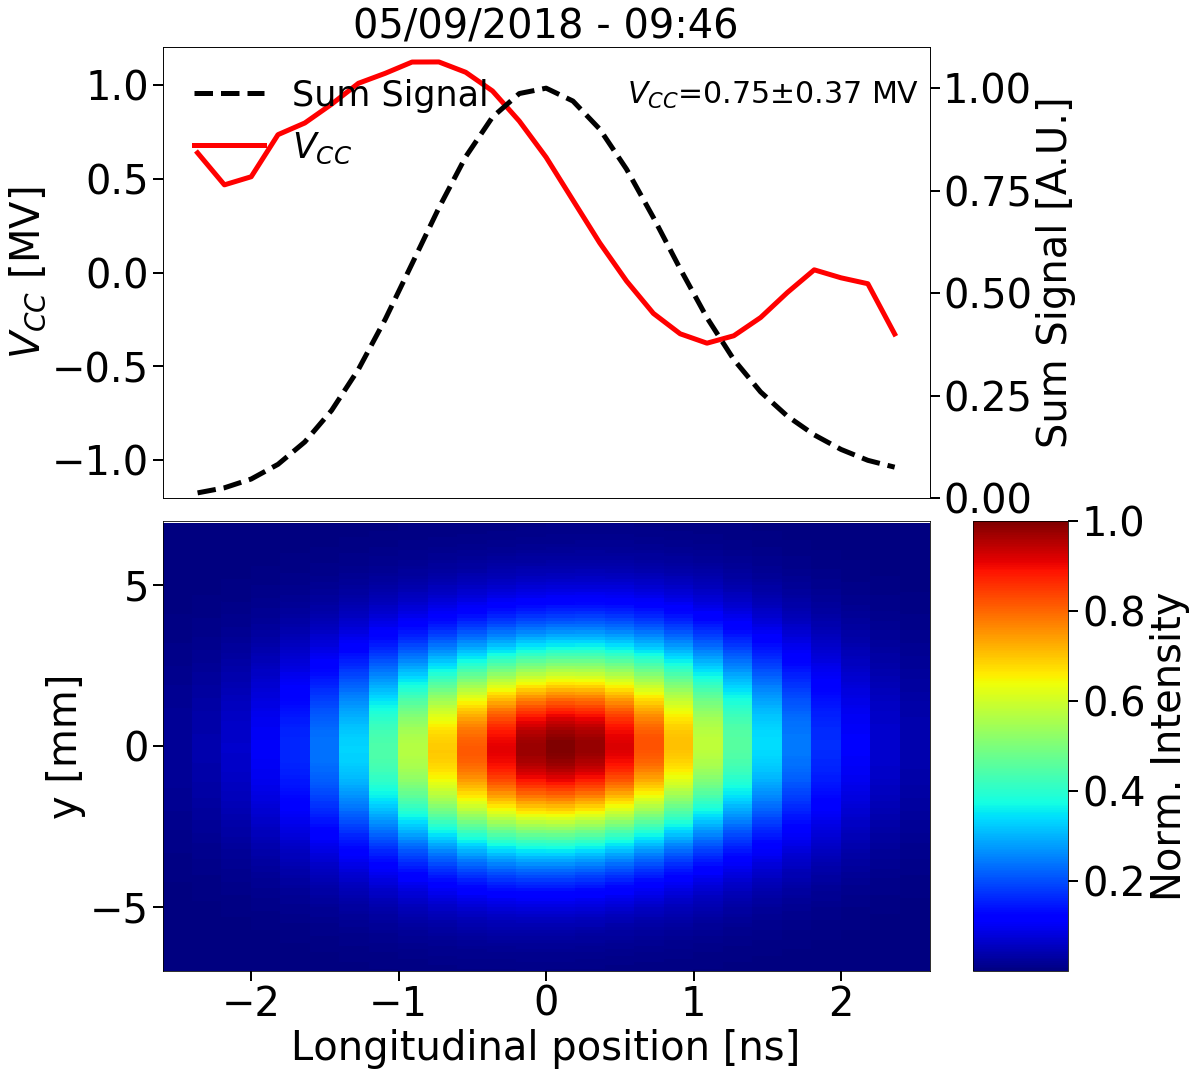
\includegraphics[width=1\textwidth]{images/Ch5/HT_crabVoltage__20180905_094640_crabbing_only.png}
        \caption{$y=\sin(2 \pi f t),\ f=50$ Hz}
        \label{fig:signal_and_DFT_example_a}
    \end{subfigure}
    \hfill
    \begin{subfigure}[t]{0.45\textwidth}
        \centering
        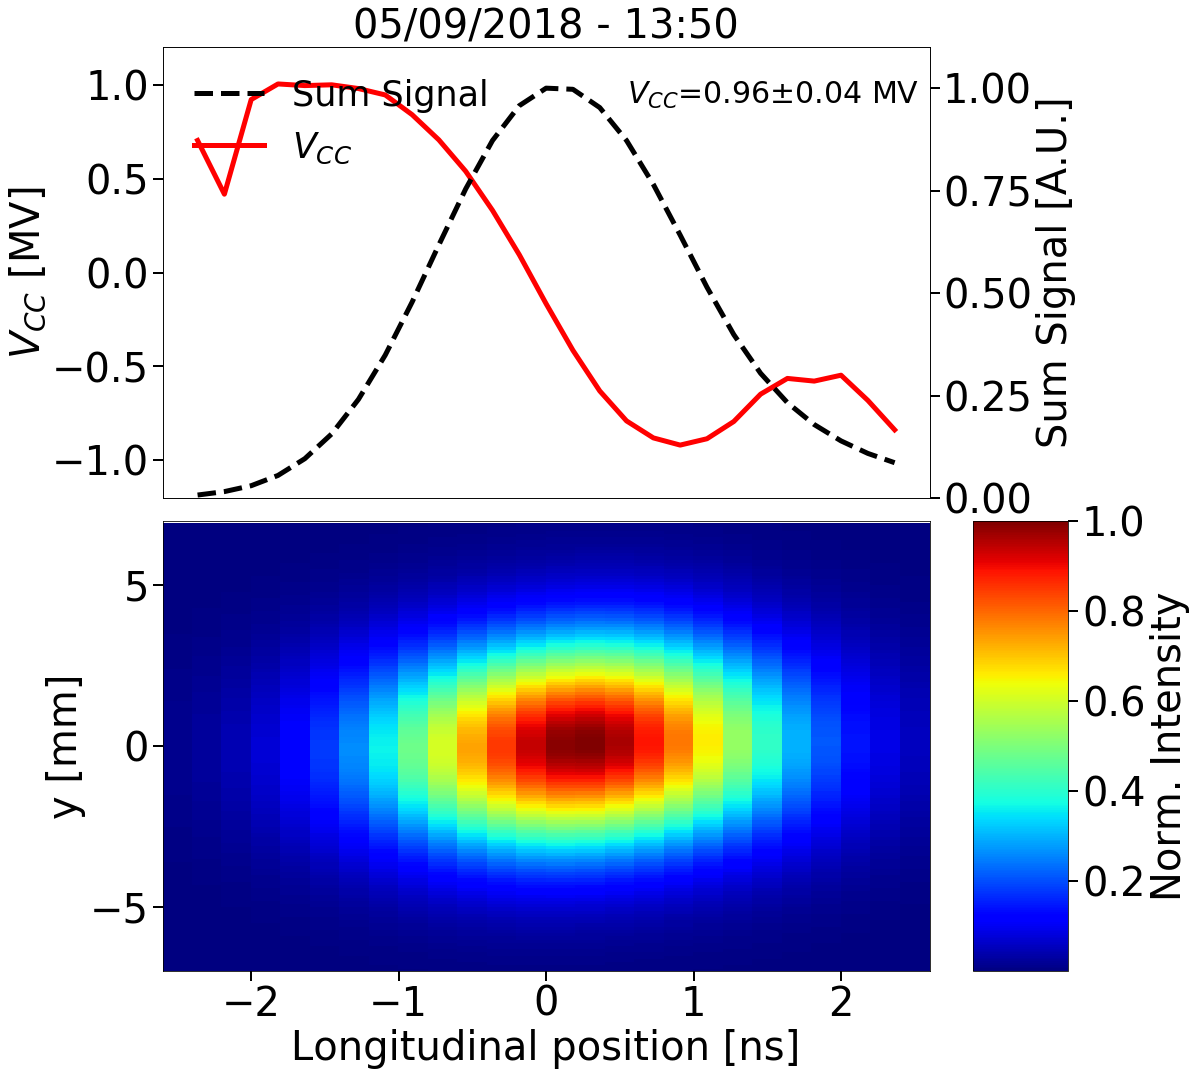
\includegraphics[width=1\textwidth]{images/Ch5/HT_crabVoltage__20180905_135033_crabbing_only.png}
        \caption{Discrete Fourier transform}
        \label{fig:signal_and_DFT_example_b}
    \end{subfigure}
    \hfill
     \caption{Example of a signal sampled at discrete time intervals, and the corresponding discrete Fourier transform.}
     \label{fig:signal_and_DFT_example}
\end{figure}




At can be seen that the signals are assymetric. Especially the first one. From the peak to peak amplitude Vcc is estimated at 0.76 MV at the first acquisition and 0.97 at the second. (We may exclude the first one as its too far from the actual coast? also in the meanwhile we had to damp the beam as some cavites (not the CC tripped)). 

For the comparison with the theory (section).. and the simulations with the realistic machine conditions (ch... with impedance), the average of these two measuremnts will be used. The uncertainty of the measurement is their (standard deviation + the unceratinties from the individual computations)

- Crabbin much less visible due to larger energy.

- We assumed that the CC settings didnt change throught the coast.
- The experts appear to be confident that the voltage was 1 MV.


- Unfortunately not many measurements are available. The closer to the start of the coast is at 9:46 which is actually from the previous coast. we asssume tha the setting remain the same.


- For the analysis here it is assumed that the voltage remained unchanged through the experiment. 
- peak to peak for non symmetric signals.
- High uncertainty due to the coast at 270 GeV
- The experts appear to be confident.

\section{Injected RF noise}\label{sec:noise_meas2018}
\begin{sloppypar} % to fix \hbox too wide
 The injected noise was a mixture of amplitude and phase noise up to 10\,kHz, overlapping and primarily exciting the first betatron sideband at $\sim 8$\,kHz. The phase noise was always dominant. Figure~\ref{fig:example_PN_and_AN} dsiplays two example measurements of phase (left) and amplitude (right) noise acquired during the experiment with a sepctrum analyzer E5052B~\cite{E5052B_insight}. 
\end{sloppypar} 

 % Loaction for creating the figure: /cernbox/2020/injected_noise_MD5_2018
 \begin{figure}[!ht]
    \centering
    \begin{subfigure}[t]{0.45\textwidth}
        \centering
        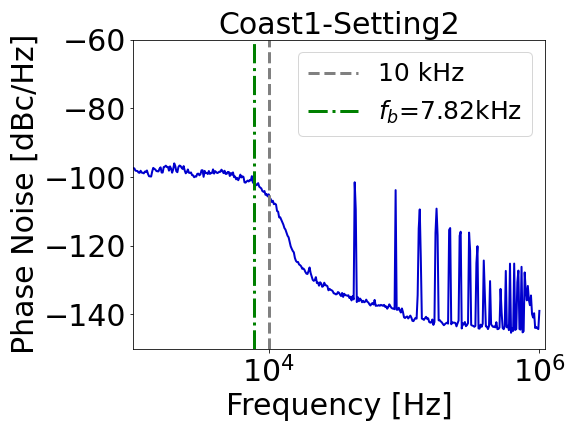
\includegraphics[width=1\textwidth]{images/Ch5/Measured_spectrum_MD5_Coast1-Setting2-PN.csv_no_psd.png}
        %\caption{$y=\sin(2 \pi f t),\ f=50$ Hz}
        %\label{fig:add_label_here}
    \end{subfigure}
    \hfill
    \begin{subfigure}[t]{0.45\textwidth}
        \centering
        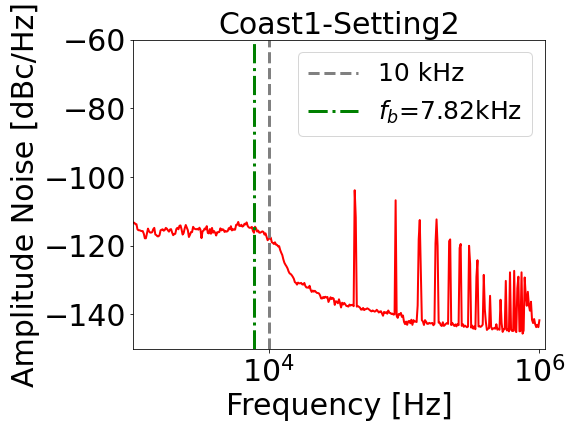
\includegraphics[width=1\textwidth]{images/Ch5/Measured_spectrum_MD5_Coast1-Setting2-AN.csv_no_psd.png}
        %\caption{Discrete Fourier transform}
        %\label{fig:add_label_here}
    \end{subfigure}
    \hfill
     \caption{Example phase (left) and amplitude (right) noise spectra measured with a spectrum analyzer E5052B during the emittance growth studies with CCs in SPS. The noise spread-out up to 10\,kHz (grey dashed line) exciting the first betatron sideband at $\sim$8\,kHz (green dashed line). The spikes at high frequencies correspond to the harmonics of the revolution frequency and are a result of the bunch crossing.} % bunch passage
     \label{fig:example_PN_and_AN}
\end{figure}

\begin{sloppypar} % to fix \hbox too wide
This spectrum analyzer provides a single sideband measurement (SSB), which is expressed as $10\log_{10}\mathcal{L}(f)$\,[dBc/Hz]. Its relation with the power spectral densities (PSDs) introduced in Eq.~\eqref{eq:dey_an} and Eq.~\eqref{eq:dey_pn} are given by $S_\Delta = 2\mathcal{L}(f)$~\cite{IEEE:4797525}, with $S_{\Delta A}$ in 1/Hz and $S_{\Delta\phi}$ in rad$^2$/Hz. A detailed discussion on the noise power measurements and their relation to the mathimatical defintion of the PSD is given in Chapter [tba].

As already mentioned above, the injected noise was a combination of both phase and amplitude noise. Therefore, in order to make a meaningful comparison between the different noise levels the concept of effective phase noise is introduced. This is the phase noise level that would lead to
the same emittance growth as that from both phase and
amplitude noise. The noise levels mentioned in this Chapter correspond to the calculated effective phase noise.
% should I slightly change this paragraph? Too much copy paste from IPAC or it's ok?
\end{sloppypar} 

\section{Emittance growth measurements}\label{sec:EmitGrowth_measurements}
% Figures for emit growth evolution MD 2018: SWAN_projects/CC_MDs_2018/myAnalysis_2020/for_thesis/average_MD5_overview_5Sep2018_emitBU_PlotOverview_Vertical_OpenRatesFromPickle_for_thesis.ipynb


MD emittance growth overview. 
    - average from IN and OUT. As mentioned in CH4. vs time and vs noise level for all bunches. Not yet comparison with the theory. Probably you need to re-run this to make correctly the error propagation. 
    - 1 noise point was excluded
 


\section{Bunch length measurements}\label{sec:bunch_length_measurements_2018}
    - bunch length and longitudinal profiles and relative position from the wall current monitor.  unstable bunches.
    - bunch 2-3-4 longutidinally unstable.
 
\section{Intensity measurements}\label{sec:intensity_measurements_2018}
No losses. Maybe not seperate chapter?
I should also mention in Ch4 how the emittance is measured from the ABWLM.

\section{Comparison of measured emittance growth with the theory}\label{sec:meas_2018_vs_theory}

Comparison of bunch 1 with theory. Discrepancy of a factor 4.


 \section{Conclusions and outlook}\label{sec:MD2018_summary}
